% Compilar desde esta carpeta: tectonic informe.tex
% Alternativa: latexmk -pdf -interaction=nonstopmode -halt-on-error informe.tex
\documentclass[11pt,a4paper]{article}
\usepackage[utf8]{inputenc}
\usepackage[T1]{fontenc}
\usepackage[spanish,es-tabla,es-noshorthands]{babel}
\usepackage{lmodern}
\usepackage[a4paper,margin=1.85cm,headheight=14pt,headsep=6mm,footskip=10mm]{geometry}
\usepackage{microtype,graphicx,booktabs,tabularx,array,amsmath,amssymb}
\usepackage[dvipsnames]{xcolor}
\usepackage{tikz}
\usetikzlibrary{arrows.meta,positioning,shapes.geometric}
\usepackage{caption,enumitem,fancyhdr,titlesec}
\usepackage[hidelinks,unicode]{hyperref}
\definecolor{ink}{HTML}{183748}
\definecolor{accent}{HTML}{B85130}
\definecolor{pale}{HTML}{EDF3F5}
\hypersetup{pdftitle={ProductShot AI: informe técnico},pdfauthor={Aaron Camacho, Nicolas Castañeda, Isaac Vera, Pedro Mori, Juan Diego Castro},pdfsubject={Proyecto 2, Planificación y Toma de Decisiones en IA}}
\pagestyle{fancy}\fancyhf{}
\fancyhead[L]{\small\textcolor{ink}{\textbf{ProductShot AI}}}
\fancyhead[R]{\small CS5363 \textperiodcentered{} UTEC \textperiodcentered{} 2026-2}
\fancyfoot[R]{\small\thepage}
\renewcommand{\headrulewidth}{0.3pt}
\titleformat{\section}{\Large\bfseries\color{ink}}{\thesection.}{0.6em}{}
\titleformat{\subsection}{\normalsize\bfseries\color{ink}}{\thesubsection}{0.5em}{}
\titlespacing*{\section}{0pt}{0pt}{9pt}
\titlespacing*{\subsection}{0pt}{9pt}{4pt}
\setlength{\parindent}{0pt}\setlength{\parskip}{6pt}
\setlength{\emergencystretch}{2em}
\setlist[itemize]{leftmargin=*,nosep,topsep=3pt}
\captionsetup{font=small,labelfont=bf,skip=5pt}
\newcolumntype{Y}{>{\raggedright\arraybackslash}X}
\newcommand{\ruta}[1]{{\small\texttt{\detokenize{#1}}}}
\newcommand{\foto}[2]{\begin{minipage}[t]{0.315\linewidth}\centering\includegraphics[width=\linewidth]{figures/#1}\\[-1pt]{\small #2}\end{minipage}}
\begin{document}

% ---------------- Página 1 ----------------
{\LARGE\bfseries\color{ink} ProductShot AI}\par
{\large Generación de ambientaciones para fotografía de producto}\par
\textbf{Proyecto 2 \textperiodcentered{} Planificación y Toma de Decisiones en IA}\par
\textbf{Integrantes:} Aaron Camacho, Nicolas Castañeda, Isaac Vera, Pedro Mori, Juan Diego Castro\par
\textbf{Docente:} Robert Junior Buleje Del Carpio\par

\subsection*{Resumen}
ProductShot AI recibe la foto de un producto y genera cinco ambientaciones para que una persona elija cuáles usaría. El sistema une segmentación, generación de imágenes, controles de fidelidad, registro de decisiones y un resumen escrito por un modelo de lenguaje. Tiene dos modos: el intermedio edita la foto con Qwen-Image-2.1-Turbo y el avanzado rellena el fondo con SDXL y un adaptador LoRA propio. Este informe describe el diseño, la implementación y los resultados obtenidos. En una prueba local con una taza de cerámica mate, el sistema produjo cinco imágenes reales; se aceptaron cuatro y el resumen pasó la verificación de estructura. También contamos con los registros de curación de datos y con la comparación de configuraciones del modo avanzado. Estos resultados muestran que el sistema funciona de principio a fin, pero todavía no permiten afirmar que sea útil en general, que satisfaga a sus usuarios ni que un modo supere al otro.

\section{Problema, objetivos y alcance}
Muchas personas venden productos con fotos tomadas en casa, sin estudio fotográfico ni experiencia en edición. El reto no es solo producir fondos atractivos: una foto de venta debe mostrar el producto tal como es, con su forma, su etiqueta y su logotipo. Que esta herramienta resuelva una necesidad real, y que la gente la acepte, son hipótesis que todavía hay que contrastar con usuarios.

El objetivo es obtener \textbf{exactamente cinco variaciones por ronda}, una por estilo (estudio, natural, cálido, lifestyle y minimalista), dejar que la persona acepte o rechace cada una y resumir sus decisiones sin inventar nada. El sistema admite hasta tres rondas, y cada ronda nueva se ajusta según las decisiones anteriores. No reconstruye caras ocultas del producto ni su forma en 3D. El alcance inicial se limita a un solo producto pequeño, rígido y de preferencia opaco.

La tabla resume las etapas del proyecto y lo que respalda cada una.

\begin{table}[h]\centering\small
\begin{tabularx}{\linewidth}{@{}p{2.8cm}YY@{}}\toprule
Etapa & Trabajo realizado & Respaldo \\\midrule
Definición & Alcance, cinco estilos y decisión por imagen & Modelo de dominio y configuración \\
Diseño & API, contratos y adaptadores intercambiables & Servicios y worker HTTP \\
Prototipo & Flujo completo con generación simulada & Backend simulado y pruebas automáticas \\
Generación & Edición con Qwen y adaptación SDXL--LoRA & Imágenes generadas y revisión ciega \\
Interacción & Web móvil, Gradio, rondas y resumen & Interfaz y sesión guardada \\
Evaluación & Pruebas técnicas y protocolo con usuarios & Pruebas; entrevistas pendientes \\\bottomrule
\end{tabularx}
\end{table}
En las secciones siguientes separamos tres cosas: lo que está implementado, lo que se ejecutó y midió, y lo que aún falta evaluar.

\clearpage
% ---------------- Página 2 ----------------
\section{Arquitectura y decisiones técnicas}
El sistema separa la interacción, las reglas de la aplicación, el almacenamiento y la inferencia. FastAPI expone la API en \ruta{/api/v1}, y las dos interfaces, la web en \ruta{/app} y Gradio en \ruta{/ui}, la consumen por HTTP. El servicio de sesiones controla los estados y envía las solicitudes a adaptadores que se eligen por configuración. Los modelos pesados corren en workers de Modal, así que la API no necesita GPU.

\begin{figure}[h]\centering
\begin{tikzpicture}[font=\small,node distance=8mm and 10mm,
 b/.style={draw=ink,rounded corners=3pt,fill=pale,align=center,text width=4.4cm,minimum height=11mm},
 a/.style={-{Stealth[length=2mm]},thick,draw=ink}]
\node[b] (ui) {Persona usuaria\\Web HTML/CSS/JS o Gradio};
\node[b,below=of ui] (api) {FastAPI + servicio de sesiones\\validación, estados y trabajos};
\node[b,left=of api,text width=3.3cm] (db) {SQLite + archivos\\retención: 24 h\\desde la primera ronda};
\node[b,right=of api,text width=3.3cm] (llm) {Gemini\\solo decisiones y motivos};
\node[b,below left=12mm and 4mm of api,text width=5.6cm] (qwen) {Worker intermedio \textperiodcentered{} Modal\\BiRefNet + controles + Qwen\\H100 / A100 de 80 GB};
\node[b,below right=12mm and 4mm of api,text width=5.6cm] (sdxl) {Worker avanzado \textperiodcentered{} Modal\\SDXL inpainting + LoRA + control\\L4 / A10G};
\draw[a,<->] (ui)--node[right]{HTTP} (api);
\draw[a,<->] (api)--(db);
\draw[a,<->] (api)--(llm);
\draw[a,<->] (api)--(qwen);
\draw[a,<->] (api)--(sdxl);
\end{tikzpicture}
\caption{Arquitectura del sistema. La limpieza de datos corre en la API al arrancar y cada diez minutos. Las GPU indicadas son las que usa cada worker; el modo avanzado también usa la segmentación del worker intermedio.}
\end{figure}

\begin{table}[h]\small
\begin{tabularx}{\linewidth}{@{}p{3.0cm}YY@{}}\toprule
Decisión & Motivo & Costo que aceptamos \\\midrule
Puertos y adaptadores & Cambiar simulaciones por servicios reales y probar sin GPU & Más contratos y validación entre procesos \\
SQLite y archivos & Implementación simple; cada sesión queda trazable & Sin base distribuida ni alta disponibilidad \\
Workers separados & Qwen y SDXL necesitan dependencias y memoria distintas & Dos entornos y dos arranques en frío \\
Modal y contenedor API & Separar el cómputo con GPU del servidor web & Dependencia de la red y de los proveedores \\
Resumen estructurado & Comparar IDs, decisiones y citas con el registro & La prosa libre solo se revisa en parte \\\bottomrule
\end{tabularx}
\end{table}

\subsection{Datos, estados y recuperación}
La base de datos relaciona sesiones, fotos de entrada, máscaras, trabajos de generación, variaciones, decisiones y resúmenes. Cada variación guarda su semilla, la revisión del modelo, la versión del prompt y sus parámetros. Una ronda nueva guarda la sesión de la que viene y el plan que la produjo. Con esta información se puede reconstruir cada resultado y explicar por qué el sistema lo generó.

Una sesión sigue los estados \texttt{UPLOADED} $\rightarrow$ \texttt{SEGMENTED} $\rightarrow$ \texttt{GENERATING} $\rightarrow$ \texttt{READY\_FOR\_REVIEW} $\rightarrow$ \texttt{REVIEWED} $\rightarrow$ \texttt{SUMMARIZED}. Si algo falla, queda en \texttt{FAILED}. La API acepta claves de idempotencia para no crear trabajos duplicados. El ejecutor local usa un hilo, de modo que un reinicio interrumpe el trabajo en curso y no lo retoma.

La retención (G11) se controla con \ruta{SESSION_RETENTION_HOURS=24} y una revisión cada 600 segundos. Cuando la primera ronda cumple el plazo, se borran los registros y las carpetas de toda la cadena; crear rondas nuevas no reinicia el plazo. Si hay una generación activa, el borrado espera; si el lote quedó colgado, G14 lo marca como fallido y deja de bloquear. Un contenedor Docker permite desplegar la API en un servicio como Railway, y los datos persisten si se monta un volumen.

\clearpage
% ---------------- Página 3 ----------------
\section{Modelos generativos y conservación del producto}
\subsection{Modo intermedio: edición por instrucciones}
Este modo carga \texttt{Qwen/Qwen-Image-2.1-Turbo} con \texttt{QwenImage21Pipeline}, en precisión \texttt{bfloat16}, y hace ocho pasos por candidata. El modelo edita una imagen a partir de la propia imagen y de un texto~\cite{qwen}. El sistema arma la instrucción de escena con el estilo, la categoría del producto y un conjunto cerrado de ajustes. La imagen se lleva a cerca de un megapíxel para generar y luego se devuelve al tamaño de trabajo.

A diferencia del inpainting, que pega de nuevo el producto original, este modo puede cambiar toda la imagen y adaptar la luz del objeto a la escena. Por eso la máscara de BiRefNet no se entrega al editor: se usa después, para verificar la fidelidad. De ahí viene tanto la mejor integración visual como el riesgo de que cambien etiquetas o detalles.

Por cada estilo se generan hasta tres candidatas. La verificación alinea el producto con puntos ORB y RANSAC, y mide las correspondencias, los bordes y el cambio de fondo. Una candidata $c$ es válida si cumple:
\[
\operatorname{válida}(c)=\operatorname{alineada}(c)\land
r_{\mathrm{inliers}}\geq0.45\land\rho_{\mathrm{bordes}}\geq0.40
\land\Delta_{\mathrm{fondo}}\geq25.
\]
Aquí $r_{\mathrm{inliers}}$ es la proporción de correspondencias consistentes, $\rho_{\mathrm{bordes}}$ la correlación entre mapas de bordes de Sobel y $\Delta_{\mathrm{fondo}}$ la diferencia de intensidad del fondo, en escala de 0 a 255. Entre las candidatas válidas se elige la que maximiza $r_{\mathrm{inliers}}\max(0,\rho_{\mathrm{bordes}})$. La SSIM normalizada se registra para diagnóstico, pero no decide.

Si ningún candidato de un estilo es válido, el sistema reintenta mientras la latencia p95 observada quepa en un presupuesto de 420 segundos. Si al final falta un estilo, falla el lote completo. Así se cumple la promesa de cinco imágenes, aunque a veces el servicio no responda. Pasar estos umbrales no asegura que el texto, la marca o las propiedades físicas del producto sean exactos.

\subsection{Modo avanzado: SDXL con LoRA}
SDXL es un modelo de difusión latente: un VAE comprime la imagen en un espacio latente, y una red condicionada por texto elimina ruido de esos latentes hasta producir una imagen~\cite{sdxl}. El worker avanzado usa el checkpoint \texttt{diffusers/stable-diffusion-xl-1.0-inpainting-0.1}, que recibe nueve canales: los latentes con ruido, la máscara y los latentes de la imagen enmascarada~\cite{inpaint}.

LoRA adapta las matrices del modelo con una actualización de bajo rango,
\[
W'=W_0+sBA,\qquad A\in\mathbb{R}^{r\times d},\quad
B\in\mathbb{R}^{k\times r},\quad r\ll\min(k,d),
\]
y deja congelados los pesos base~\cite{lora}. Así se entrena una fracción pequeña de los parámetros. Implementamos tres variantes de entrenamiento: la estándar, una con pérdida solo sobre el fondo y otra con objetivo de inpainting. Cada corrida guarda un manifiesto que indica qué variante produjo el adaptador.

La configuración que sirve el modo avanzado usa el adaptador \texttt{v5distill-ckpt1000}, prompts v2, peso LoRA 1, intensidad de cambio 1, 30 pasos y guía 7. El lienzo limita la altura del producto al 45\,\% y apoya su base al 85\,\%. Después de generar, el control G8 vuelve a pegar los píxeles protegidos del producto. El interior de la máscara se conserva, aunque los bordes suaves, la segmentación y el reencuadre pueden introducir diferencias.

\textbf{Comparabilidad.} Los dos modos usan modelos y formas de conservar el producto distintas, así que una diferencia entre ellos no se puede atribuir solo a LoRA. Para medir su efecto hay que comparar SDXL con y sin el adaptador, con la misma configuración.

\clearpage
% ---------------- Página 4 ----------------
\section{Datos, entrenamiento y selección del adaptador}
\subsection{Curación y partición de datos}
La preparación de BG60k incluye manifiestos de imágenes y máscaras, filtros de calidad, detección de duplicados, clasificación por estilo y revisión visual. En el piloto se aceptan imágenes con un producto dentro del alcance y una ambientación acorde al estilo; se rechazan, entre otras, las de fondo incorrecto, varios productos u objetos transparentes o muy reflectantes. BG60k solo permite uso académico~\cite{bg60k}.

La partición final tiene 257 registros: 209 para entrenamiento, 23 para validación y 25 para prueba. Para que un mismo producto no aparezca en dos particiones, combinamos búsqueda por similitud con revisión manual de identidad. La auditoría registra 589 decisiones de revisión y dos coincidencias que obligaron a mover grupos de imágenes; una revisión final de 93 pares no encontró más casos. Esto reduce el riesgo de fuga de datos, pero no lo elimina.

\begin{table}[h]\centering
\caption{Partición final después de la revisión.}
\begin{tabular}{@{}lrrrr@{}}\toprule
Estilo & Entrenamiento & Validación & Prueba & Total \\\midrule
Estudio & 36 & 4 & 4 & 44 \\
Natural & 42 & 5 & 5 & 52 \\
Cálido & 36 & 3 & 4 & 43 \\
Lifestyle & 48 & 6 & 6 & 60 \\
Minimalista & 47 & 5 & 6 & 58 \\\midrule
Total & 209 & 23 & 25 & 257 \\\bottomrule
\end{tabular}
\end{table}

Cada caption combina la descripción del estilo con el nombre del producto. También usamos autodestilación: el modelo genera candidatas, se conservan las que cumplen el estilo según CLIP y tienen una similitud DINOv2 del producto de al menos 0.9, se aplican exclusiones visuales y se exporta un conjunto con imágenes, máscaras y captions. \textbf{Los 257 registros de la tabla no son el tamaño del conjunto destilado}; ese tamaño no quedó registrado.

\subsection{Entrenamiento}
El entrenamiento corre en Colab y se controla desde la línea de comandos. El controlador revisa que no haya máquinas activas, sube los datos y la configuración, ejecuta el trabajo, descarga los resultados y libera la máquina. Registra versiones, hashes de scripts y pesos, uso de memoria y pérdidas. Usa el script de entrenamiento de Diffusers 0.31.0, verificado por SHA-256, con cambios explícitos para las variantes de pérdida e inpainting. Un presupuesto de tiempo y la limpieza al final evitan gastar créditos por accidente.

Por defecto, el controlador usa rango 16 y tasa de aprendizaje $10^{-4}$, con lote de una imagen, acumulación de gradientes configurable y \emph{gradient checkpointing}. Estos son los valores por defecto, \textbf{no los confirmados para la corrida final}: no conservamos el manifiesto, los pesos intermedios ni las curvas del adaptador elegido. Por eso no reportamos pérdida final, costo, duración ni memoria como resultados medidos.

\subsection{Selección del adaptador}
En la revisión ciega comparamos \texttt{v4\_ckpt400\_v1} con \texttt{v5\_ckpt1000\_v2}: en 15 pares, v5 fue preferido 8 veces, v4 2 veces y en 5 no hubo preferencia. En un conteo aparte de imágenes con equipo de estudio visible, v4 lo mostró en 13 de 15 casos y v5 en 0 de 15. Esto respalda la elección de v5, pero tiene límites: entre ambas versiones cambian a la vez el checkpoint y los prompts, y los evaluadores no fueron una muestra independiente. No es una prueba de superioridad general ni una prueba con usuarios.

\clearpage
% ---------------- Página 5 ----------------
\section{Flujo del sistema e interfaz}
\begin{figure}[h]\centering
\begin{tikzpicture}[font=\scriptsize,
 n/.style={draw=ink,rounded corners,fill=pale,align=center,minimum height=10mm,text width=2.55cm},
 a/.style={-{Stealth[length=1.7mm]},thick,draw=ink}]
\node[n] (a) at (0,0) {1. Foto, categoría\\y modo};
\node[n] (b) at (3.25,0) {2. Controles\\y segmentación};
\node[n] (c) at (6.5,0) {3. Generar y validar\\cinco salidas};
\node[n] (d) at (9.75,0) {4. Aceptar/rechazar\\cada imagen};
\node[n] (e) at (13,0) {5. Validar resumen\\y mostrar resultado};
\foreach \x/\y in {a/b,b/c,c/d,d/e} \draw[a] (\x)--(\y);
\draw[a] (e.south)--++(0,-0.5) -| node[pos=.25,below]{Otra ronda: decisiones + ajustes por reglas; máximo 3} (c.south);
\end{tikzpicture}
\caption{Flujo normal. Si la foto se rechaza o el lote queda incompleto, el sistema muestra un error. El borrado, manual o por retención, elimina toda la cadena de rondas.}
\end{figure}

La web está hecha con HTML, CSS y JavaScript, y tiene cuatro pantallas: Foto, Crear, Elegir y Listo. Permite usar la cámara o la galería, reduce el tamaño de la imagen y consulta el estado cada 2.5 segundos. Guarda las decisiones y los motivos antes de pedir el resumen. Gradio permite además ver y reemplazar la máscara. Las dos interfaces avisan el plazo de borrado: la web lo consulta a la API y Gradio lo recibe al iniciar.

\begin{figure}[h]\centering
\begin{minipage}[c]{0.30\linewidth}\centering

\includegraphics[height=11.1cm]{figures/ui_upload.png}
\end{minipage}\hfill
\begin{minipage}[c]{0.63\linewidth}\centering

\includegraphics[width=0.78\linewidth]{figures/ui_decision_detail.png}\par\vspace{4mm}
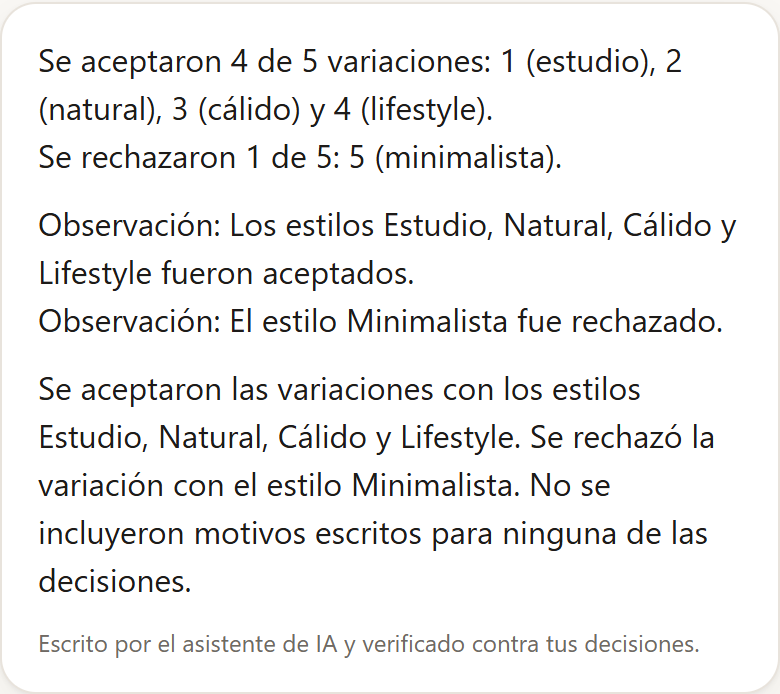
\includegraphics[width=0.78\linewidth]{figures/ui_summary_detail.png}
\end{minipage}
\caption{Interfaz móvil: selección de foto, decisión sobre una imagen y resumen. Capturas de la sesión de prueba con la taza.}
\end{figure}

\textbf{Resumen y rondas.} Gemini recibe solo las decisiones y los motivos, y devuelve un JSON con estructura fija. Python verifica que cubra las cinco variaciones y que los IDs, las etiquetas y las citas coincidan con el registro; la lista de decisiones se arma desde la base de datos. Si Gemini falla, se prueba un modelo de respaldo y, si también falla, se usa un resumen armado sin LLM. La narración libre solo se valida en parte y no debe suponer motivos que la persona no escribió. Las rondas siguientes las planifica un conjunto de reglas con un vocabulario cerrado de ajustes; no las decide un LLM.

\textbf{Mejoras pendientes en la interfaz.} El progreso que se muestra es una estimación. Frases como ``listas para vender'' o ``verificado por el asistente'' prometen demasiado: conviene revisarlas y distinguir la validación de estructura de la de contenido. El aviso de retención también debería decir que el borrado ocurre en revisiones periódicas.

\clearpage
% ---------------- Página 6 ----------------
\section{Ejemplos de imágenes y decisiones}
Hicimos una prueba local con una taza de cerámica mate, con el modo intermedio y la categoría cocina. La taza es rígida y opaca, como los productos del alcance. Las cinco imágenes son salidas reales de Qwen. Las guardamos aparte junto con sus hashes y parámetros, para que la retención no las borre.

\begin{figure}[h]\centering
\foto{input.png}{(a) Fotografía de entrada}\hfill
\foto{variation_1.png}{(b) Estudio \textperiodcentered{} aceptada}\hfill
\foto{variation_2.png}{(c) Natural \textperiodcentered{} aceptada}
\par\vspace{7pt}
\foto{variation_3.png}{(d) Cálido \textperiodcentered{} aceptada}\hfill
\foto{variation_4.png}{(e) Lifestyle \textperiodcentered{} aceptada}\hfill
\foto{variation_5.png}{(f) Minimalista \textperiodcentered{} rechazada}
\caption{Taza de cerámica mate: foto de entrada y las cinco ambientaciones generadas. Se aceptaron cuatro y se rechazó la minimalista, sin motivos escritos. Es una prueba interna, no una entrevista con participantes.}
\end{figure}

En todas se reconocen la silueta, el borde claro y el cuerpo oscuro de la taza; la versión natural agrega una mesa de madera y luz lateral. Sin embargo, las versiones de estudio y minimalista agregan marcas al frente que no están en la foto original. Ambas pasaron el filtro automático y la de estudio fue aceptada: pasar las métricas o gustar no asegura que el producto se conserve por completo.

\textbf{Qué permite concluir este ejemplo.} La foto muestra un solo producto, con el asa en parte oculta y sin texto visible. Sirve para detectar elementos agregados, pero no para evaluar si se conservan etiquetas existentes. No sabemos por qué se rechazó la versión minimalista. Tampoco tenemos todavía ejemplos del modo avanzado con sus parámetros registrados.

\clearpage
% ---------------- Página 7 ----------------
\section{Análisis de resultados técnicos}
\subsection{Sesión de prueba}
La generación de las cinco imágenes duró \textbf{298.7 segundos}, casi cinco minutos, sin contar la carga, la segmentación, las decisiones ni el resumen. Se generaron \textbf{86 candidatas, con 71 reintentos}: 70 en el estilo cálido y uno en lifestyle. Las cinco imágenes elegidas superaron los umbrales; en cálido solo una de 73 candidatas fue válida.

\begin{table}[h]\centering\small
\caption{Métricas de las candidatas elegidas en la sesión de prueba.}
\begin{tabular}{@{}lrrrrl@{}}\toprule
Estilo & Inliers & Bordes & Cambio fondo & Cand./reint. & Decisión \\\midrule
Estudio & 0.664 & 0.8987 & 71.8 & 3/0 & Aceptada \\
Natural & 0.515 & 0.7525 & 86.2 & 3/0 & Aceptada \\
Cálido & 0.480 & 0.9126 & 85.0 & 73/70 & Aceptada \\
Lifestyle & 0.585 & 0.8617 & 84.3 & 4/1 & Aceptada \\
Minimalista & 0.624 & 0.8824 & 74.5 & 3/0 & Rechazada \\\bottomrule
\end{tabular}
\end{table}
\textit{Inliers} es la proporción de correspondencias consistentes; \textit{bordes}, una correlación; \textit{cambio fondo}, una diferencia de 0 a 255. La penúltima columna indica candidatas totales y reintentos. Cada imagen elegida tardó entre 2.08 y 2.11 segundos en generarse, pero ese tiempo no incluye las candidatas descartadas ni su verificación. Exigir cinco imágenes válidas multiplicó el trabajo, y no guardamos las métricas de cada descarte para explicar por qué fallaron.

El resumen quedó registrado como \texttt{llm\_validated} y \texttt{structure\_verified}. El modelo principal no respondió en dos intentos y contestó el de respaldo, \texttt{gemini-3.5-flash-lite}. La lista coincide con cuatro aceptaciones y un rechazo. Como no hubo motivos escritos, el resumen no puede explicar las preferencias. Esta sesión muestra que el respaldo funciona y que los conteos son correctos, pero no mide la exactitud del contenido del resumen en general.

\subsection{Pruebas automáticas}
La batería completa, ejecutada en Windows con Python 3.12, dio \textbf{371 pruebas aprobadas y 16 omitidas, sin fallos}, en 110 segundos. Las omitidas son catorce pruebas del entrenamiento en Colab, que solo corren en Linux o macOS, una llamada real a Gemini que es opcional y una prueba que necesita OpenCV. Estas omisiones dejan sin comprobar en Windows el control de procesos del entrenamiento; en Linux esas pruebas sí se ejecutan.

Las pruebas cubren estados, contratos, lotes, rondas, máscaras, guardrails y resúmenes. Doce de ellas revisan la retención: que el plazo cuente desde la primera ronda, que se borren los archivos y todas las rondas, que se respeten las sesiones vigentes, que se reintente si hay una generación activa, la limpieza al arrancar, la opción para desactivarla y los avisos. Usan datos temporales y modelos simulados, así que no reemplazan la revisión visual, la ejecución en GPU ni las pruebas de uso con personas.

\subsection{Qué muestran los resultados y qué falta medir}
Los resultados muestran que la generación real funciona con almacenamiento y resumen, y que existe una selección interna de la configuración del modo avanzado. No muestran una tasa de aceptación general, un ahorro frente a editar a mano ni una mejora causada por LoRA. La cifra de 4 de 5 corresponde a un solo lote: las imágenes no son participantes independientes. Además, una espera de casi cinco minutos obliga a medir cuánto tiempo tolera la gente.

La próxima evaluación debería usar varios productos dentro del alcance, guardar entradas, semillas y parámetros, y medir por separado la fidelidad, la integración visual, el estilo, la latencia y la preferencia de las personas. Para medir LoRA hay que fijar prompts, máscara y pipeline, comparar con el adaptador encendido y apagado, y dejar el conjunto de prueba fuera de la selección. Las calibraciones de umbrales hechas antes no se repitieron para este informe.

\clearpage
% ---------------- Página 8 ----------------
\section{Evaluación con usuarios}
Las entrevistas todavía no se han realizado, así que esta sección describe el protocolo previsto. Participarán unas diez personas, en sesiones de 15 a 20 minutos, y cada una hará cuatro tareas.

\begin{table}[h]\small
\begin{tabularx}{\linewidth}{@{}p{1.0cm}Yp{4.9cm}@{}}\toprule
Tarea & Actividad & Qué se registra \\\midrule
U1 & Subir una foto y preparar la generación & Éxito sin ayuda, tiempo, SEQ 1--7 \\
U2 & Decidir sobre las cinco imágenes y escribir un motivo & Éxito, tiempo, errores, aceptaciones \\
U3 & Leer el resumen y compararlo con lo decidido & Fidelidad percibida y comentario \\
U4 & Pedir y revisar otra ronda & Coherencia percibida y aceptación \\\bottomrule
\end{tabularx}
\end{table}

Cada participante recibe un código, sin registrar su nombre, y se anotan su perfil, su experiencia y el modo usado. La espera de la generación se mide aparte de las tareas. Al final se aplica el cuestionario SUS y tres preguntas abiertas. En la web la segmentación es automática y no se muestra la máscara como en Gradio, por lo que el guion se ajusta a la interfaz que se use. Al terminar, se borra la sesión; si la persona autoriza conservar su foto, se descarga antes de que venza el plazo de 24 horas y se guarda con un plazo de conservación propio.

\begin{table}[h]\small
\begin{tabularx}{\linewidth}{@{}p{5.2cm}Y@{}}\toprule
Indicador & Cómo se reporta \\\midrule
Participantes y sesiones válidas & Número total y sesiones descartadas, con su causa \\
Éxito en U1--U4 sin ayuda & Proporción por tarea con intervalo de Wilson al 95\,\% \\
Tiempo y SEQ por tarea & Mediana, rango y número de respuestas válidas \\
SUS (0--100) & Promedio, rango y número de respuestas válidas \\
Resumen fiel y ronda coherente & Conteos y explicaciones de los participantes \\
Espera, errores y ayudas & Mediana, rango y problemas observados por gravedad \\\bottomrule
\end{tabularx}
\end{table}
% Resultados de las entrevistas: completar la tabla de indicadores con los valores
% medidos, agregar una captura autorizada y relacionar 2--3 hallazgos con cambios
% de diseño concretos.

El análisis será descriptivo. Con una muestra pequeña no se afirmará representatividad ni diferencias estadísticas. Se reportarán las respuestas faltantes y los totales de cada indicador, y solo se analizarán registros con consentimiento confirmado.

\clearpage
% ---------------- Página 9 ----------------
\section{Limitaciones y consideraciones éticas}
\subsection{Fidelidad e incertidumbre}
La recomposición de SDXL protege los píxeles del producto, aunque la unión con el fondo puede verse poco natural. Qwen adapta la luz, pero puede redibujar letras o detalles, y ORB con las correlaciones no aseguran que el texto sea legible ni que la marca se conserve. El verificador también reduce las partes delgadas de la máscara, así que cables y accesorios necesitarían controles propios. Las máscaras imperfectas, los brillos, la transparencia y las oclusiones siguen siendo difíciles.

Un fondo creíble puede sugerir usos, tamaños o accesorios que el producto no incluye, y etiquetar la imagen como generada con IA no corrige eso: antes de publicar, una persona debe revisarla. La evidencia de este informe es una sesión local y revisiones internas pequeñas, con estilos desbalanceados y una curación hecha en parte con ayuda de modelos. La autodestilación además puede reforzar las preferencias del propio modelo o del evaluador automático.

\subsection{Privacidad, consentimiento y comunicación}
La foto se envía al worker remoto, y las decisiones y motivos se envían a Gemini. Al preparar la foto se quitan los metadatos EXIF, GPS y de texto PNG, y se conserva el perfil de color ICC. El consentimiento debe explicar estos recorridos y el plazo: por defecto, la cadena de rondas se borra 24 horas después de crear la primera ronda, y usar la sesión no extiende ese plazo.

El borrado se retrasa si hay una generación activa o si el servidor está apagado, y no alcanza las copias que la persona descargó, los respaldos ni los registros de los proveedores. Además, la API no autentica a los usuarios: quien conozca el ID de una sesión puede ver sus imágenes mientras existan. Borrar pronto reduce esa exposición, pero no reemplaza un control de acceso. Los filtros, por su parte, pueden confundir un dibujo estampado con un rostro o rechazar productos poco comunes; el sistema debe explicar el rechazo, y la evaluación debe contar también esos falsos positivos.

\subsection{Licencias, recursos y responsabilidad}
La licencia de Qwen permite usarlo para investigación o evaluación y pide una autorización aparte para uso comercial~\cite{qwenlicense}. BG60k solo permite uso académico~\cite{bg60k}. Por eso, aunque la idea es ayudar a preparar catálogos, el prototipo, sus datos y sus adaptadores no pueden usarse comercialmente tal como están. También hay que revisar las condiciones del checkpoint de SDXL y los derechos sobre las fotos y marcas que se suban.

Generar varias candidatas por estilo consume más cómputo. El presupuesto de tiempo, el límite de tres rondas y el apagado de contenedores inactivos acotan ese gasto, pero falta medir el costo real por sesión.

\subsection{Conclusión}
ProductShot AI une generación de imágenes, decisión humana y trazabilidad. Sus dos modos equilibran de forma distinta la integración visual y la conservación del producto, y la retención automática evita acumular fotos en el servidor. Queda pendiente completar la evidencia del LoRA, evaluar el sistema con usuarios y precisar qué garantías se comunican a quien lo usa.

\clearpage
% ---------------- Página 10 ----------------
\section{Reproducibilidad}
Esta sección resume lo necesario para ejecutar, modificar y probar el proyecto.

\textbf{Requisitos.} El proyecto usa \texttt{uv}, que instala Python 3.12 y las versiones exactas de todas las dependencias. Para la generación real hacen falta además una cuenta de Modal y una clave de Gemini de Google AI Studio.

\textbf{Modo simulado.} Con \texttt{uv sync} se instalan las dependencias y con \texttt{uv run productshot} se inicia la API junto con las dos interfaces, en \ruta{http://127.0.0.1:8000/app} y \ruta{/ui}. En este modo no se necesita GPU, red ni credenciales: la generación, la segmentación y el resumen se simulan, y cada imagen lleva una franja que lo indica. Es el modo indicado para cambiar la interfaz, el flujo o las reglas de las rondas.

\textbf{Sistema completo.} Los dos workers se despliegan en Modal con \texttt{modal deploy}; cada uno usa un token que la API también conoce. Luego se copia la plantilla de configuración a un archivo \ruta{.env} y se completan las URL de los workers, sus tokens y la clave de Gemini, y se cambian a \ruta{remote} la generación, la segmentación y la revisión de fotos, y el resumen a \ruta{gemini}. Si falta un dato, la API no arranca y explica qué falta. La ruta \ruta{/api/v1/healthz} muestra qué adaptador usa cada pieza. El adaptador LoRA no se guarda en el repositorio por su tamaño: se sube al volumen de Modal y el worker comprueba su hash antes de usarlo.

\textbf{Cambiar una pieza.} Generación, segmentación, revisión de fotos y resumen se eligen con variables de entorno. Para agregar un proveedor nuevo basta con implementar la interfaz de esa pieza y registrarla en un solo lugar del código; el orquestador sigue validando el lote de cinco, la fidelidad y el tiempo máximo. El plazo de borrado se cambia con \ruta{SESSION_RETENTION_HOURS}.

\textbf{Pruebas.} Con \texttt{uv run pytest} se ejecuta la batería completa, sin red ni GPU, porque los modelos se reemplazan por versiones simuladas. Las pruebas del entrenamiento en Colab solo corren en Linux o macOS.

\textbf{Entrenamiento.} El LoRA se entrena en Colab desde la línea de comandos, con un solo comando que reserva la GPU, entrena, verifica, descarga el resultado y libera la máquina. Cada corrida guarda un manifiesto con versiones, parámetros, pérdidas y hashes. Requiere Linux, macOS o WSL.

\textbf{Este informe.} Se compila con \texttt{tectonic informe.tex} o \texttt{latexmk -pdf informe.tex}, y usa solo figuras y diagramas TikZ locales. Después de editarlo hay que recompilar y comprobar que no pase de diez páginas.

\begingroup\small
\renewcommand{\refname}{Referencias}
\begin{thebibliography}{10}
\setlength{\itemsep}{3pt}\setlength{\parskip}{0pt}
\bibitem{qwen} Qwen. \emph{Qwen-Image-2.1-Turbo: model card}. \href{https://huggingface.co/Qwen/Qwen-Image-2.1-Turbo}{Hugging Face}. Consulta: 18/11/2026.
\bibitem{sdxl} Podell, D., et al. (2023). \emph{SDXL: Improving Latent Diffusion Models for High-Resolution Image Synthesis}. \href{https://arxiv.org/abs/2307.01952}{arXiv:2307.01952}.
\bibitem{inpaint} Diffusers. \emph{Stable Diffusion XL 1.0 Inpainting 0.1}. \href{https://huggingface.co/diffusers/stable-diffusion-xl-1.0-inpainting-0.1}{Hugging Face}. Consulta: 18/11/2026.
\bibitem{lora} Hu, E. J., et al. (2021). \emph{LoRA: Low-Rank Adaptation of Large Language Models}. \href{https://arxiv.org/abs/2106.09685}{arXiv:2106.09685}.
\bibitem{bg60k} Whileherham. \emph{BG60k}. \href{https://github.com/Whileherham/BG60k}{GitHub}. Consulta: 18/11/2026.
\bibitem{qwenlicense} Qwen. \emph{Qwen Research License Agreement}. \href{https://huggingface.co/Qwen/Qwen-Image-2.1-Turbo/blob/fc13ba1986fcb905854dc8de2f52eee395f49b5b/LICENSE}{Hugging Face}. Consulta: 18/11/2026.
\end{thebibliography}
\endgroup
\end{document}
